\section{Mel‑Scale \& Filterbanks}
\begin{frame}{}
    \LARGE \textbf{Mel‑Scale \& Filterbanks}
\end{frame}

\subsection{Perceptual Frequency Scales}
\begin{frame}[allowframebreaks]{Perceptual Frequency Scales (Human-Aware)}
    \begin{itemize}
        \item \textbf{What:}
        \begin{itemize}
            \item Human pitch perception is \textbf{non-linear}.
            \item We perceive changes at low frequencies more finely than at high frequencies.
            \item Example: Difference between 200 Hz and 300 Hz feels larger than between 3000 Hz and 3100 Hz.
        \end{itemize}
\framebreak
        \item \textbf{How:}
        \begin{itemize}
            \item Map raw frequency in Hz onto perceptual scales:
            \begin{itemize}
                \item \textbf{Mel scale} – approximates human pitch perception.
                \item \textbf{Bark scale} – based on critical bands of hearing.
                \item \textbf{ERB scale} – Equivalent Rectangular Bandwidth, linked to auditory filter widths.
            \end{itemize}
            \item Each scale compresses high-frequency regions while preserving low-frequency resolution.
        \end{itemize}
\framebreak
        \item \textbf{Why:}
        \begin{itemize}
            \item Features reflecting human hearing are more effective for \textbf{Automatic Speech Recognition (ASR)} and \textbf{Text-to-Speech (TTS)}.
            \item Speech features (e.g., MFCCs) rely heavily on perceptual scales.
        \end{itemize}

        \item \textbf{Focus: Mel Scale}
        \begin{itemize}
            \item Most widely used in speech/audio tasks.
            \item Roughly linear spacing below 1 kHz, logarithmic above.
            \item Wikipedia reference: \texttt{Mel scale page}.
        \end{itemize}
    \end{itemize}
\end{frame}

\subsection{Mel Scale}
\begin{frame}[allowframebreaks]{Mel Scale: Definition \& Intuition}

\begin{itemize}
    \item \textbf{What:}
    \begin{itemize}
        \item Mel scale converts frequency $f$ (Hz) into perceptual pitch units (mels).
        \item Forward transform:
        \[
            m = 2595 \, \log_{10}\left(1 + \frac{f}{700}\right)
        \]
        \item Inverse transform:
        \[
            f = 700 \, \left(10^{\tfrac{m}{2595}} - 1\right)
        \]
        \item Source: \texttt{Wikipedia}.
    \end{itemize}

    \item \textbf{How:}
    \begin{itemize}
        \item Use Mel spacing to set filterbank center frequencies.
        \item Commonly used in \textbf{Mel Filterbanks} and \textbf{MFCCs}.
    \end{itemize}
\framebreak

    \item \textbf{Why:}
    \begin{itemize}
        \item Aligns frequency resolution with \textbf{human pitch perception}.
        \item Compresses high-frequency regions (less perceptually important).
        \item Reduces unhelpful detail while retaining speech-relevant cues.
    \end{itemize}

    \item \textbf{Example:}
    \begin{itemize}
        \item By convention, $1000 \, \text{Hz} \approx 1000 \, \text{mels}$.
        \item Below 1 kHz: roughly linear relation.
        \item Above 1 kHz: increasingly logarithmic.
    \end{itemize}
\end{itemize}

    \begin{figure}
        \centering
        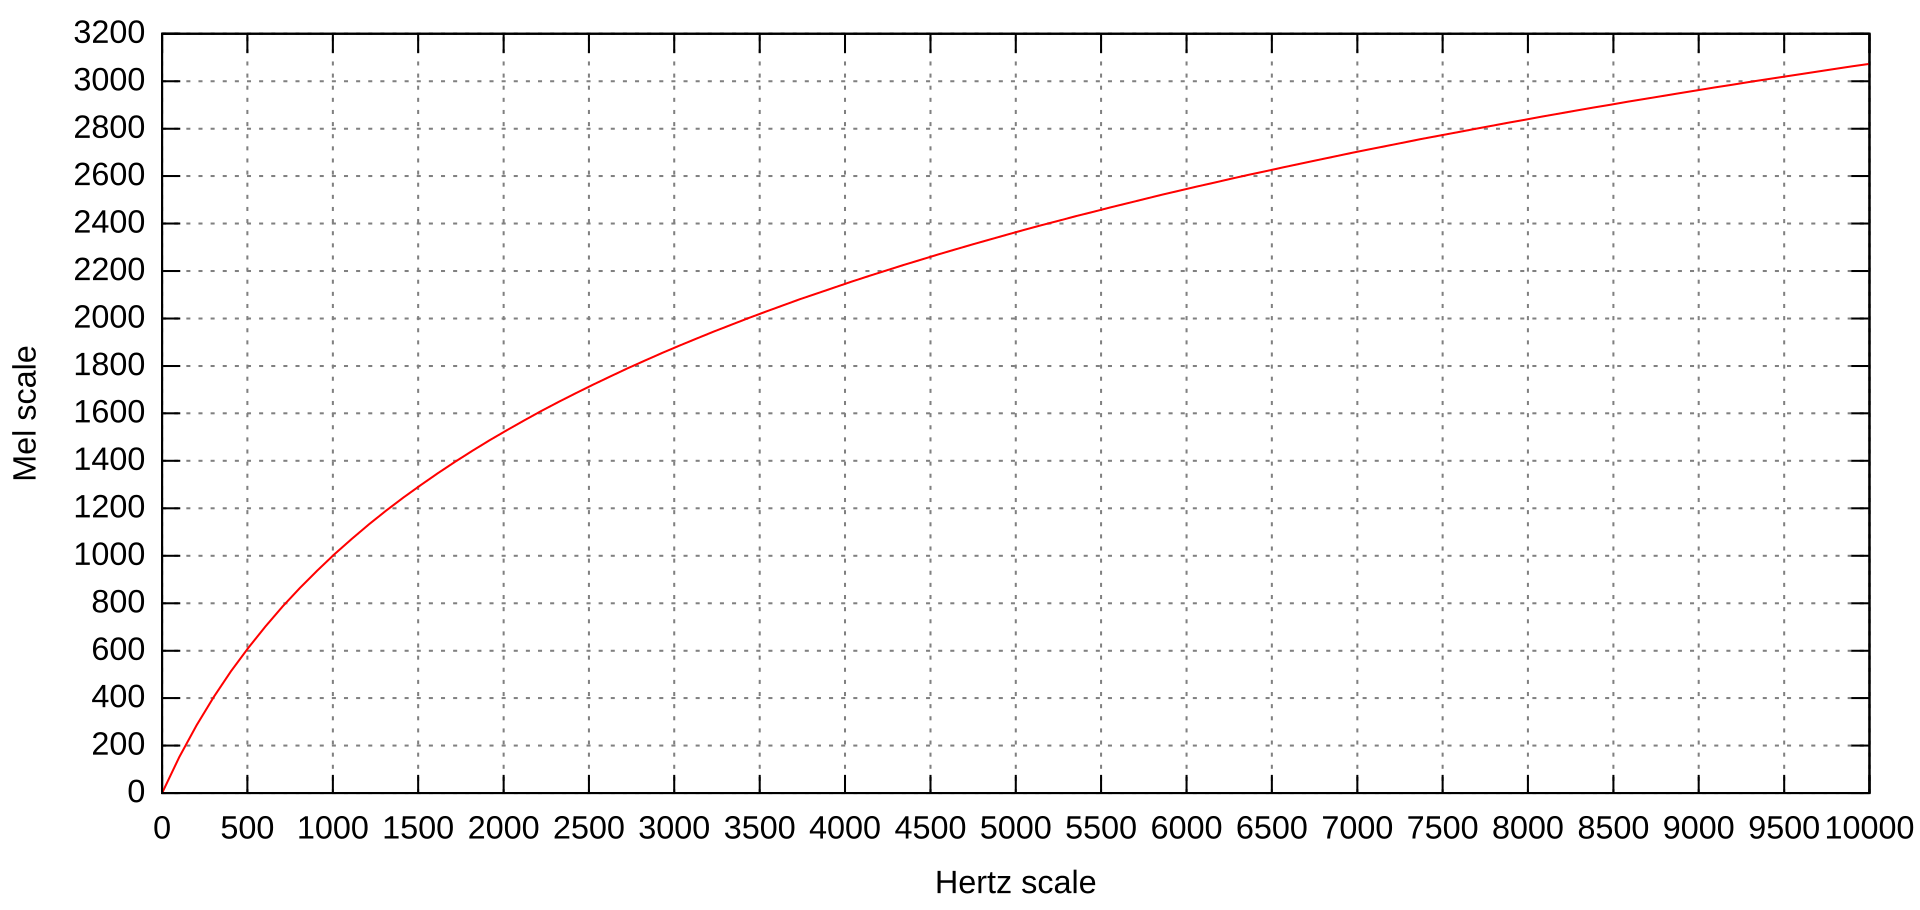
\includegraphics[width=\textwidth,height=0.8\textheight,keepaspectratio]{images/audio-nlp-eval/melscale-curve.png}
        \caption*{Plots of pitch mel scale versus hertz scale. Source: Wikipedia}
    \end{figure}

\end{frame}

\subsection{Mel Filterbanks}
\begin{frame}[allowframebreaks]{Mel Filterbanks}
    \textbf{Mel Filterbanks:} 
    \begin{itemize}
        \item The frequency axis is warped to the Mel scale.
        \item Typically, $N$ triangular filters (e.g., $N=40$) are created, spaced evenly in the Mel domain.
        \item Each filter collects energy from a range of frequencies, emphasizing perceptually important bands.
        \item The output is a set of Mel filterbank energies, which are used as features for audio and speech processing tasks.
    \end{itemize}

    \begin{figure}
        \centering
        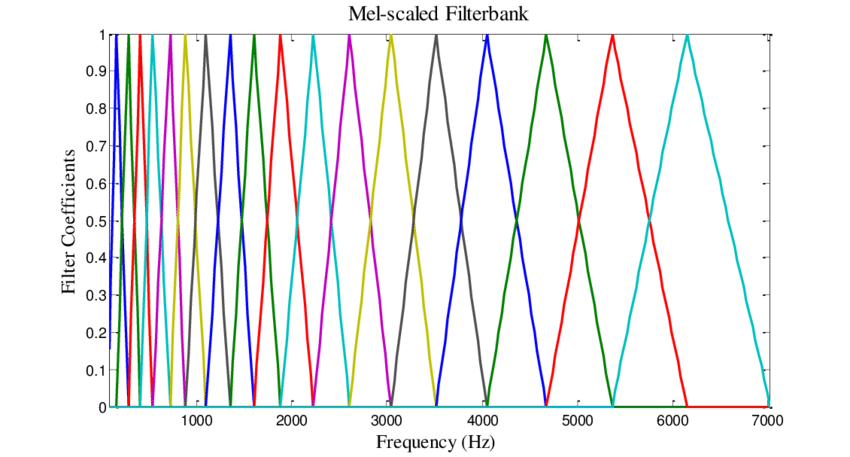
\includegraphics[width=\textwidth,height=0.8\textheight,keepaspectratio]{images/audio-nlp/mel-scaled-filterbanks.png}
    \end{figure}

\framebreak
    \textbf{Filterbank Construction Steps:}
    \begin{enumerate}
        \item Convert the lower and upper frequency bounds to Mel scale.
        \item Linearly space $N+2$ points between these bounds in Mel scale.
        \item Convert these points back to Hz to get filter edges.
        \item For each filter $k$, define a triangular response:
        \begin{equation}
            H_k(f) = 
            \begin{cases}
                0, & f < f_{k-1} \\
                \frac{f - f_{k-1}}{f_k - f_{k-1}}, & f_{k-1} \leq f < f_k \\
                \frac{f_{k+1} - f}{f_{k+1} - f_k}, & f_k \leq f < f_{k+1} \\
                0, & f \geq f_{k+1}
            \end{cases}
        \end{equation}
        \item Multiply the power spectrum by each filter and sum to get filterbank energies.
    \end{enumerate}
\end{frame}

\subsection{Choosing Features}
\begin{frame}[allowframebreaks]{Feature Families: Overview \& When to Use Which}

    \begin{itemize}
        \item Different feature types capture sound information at different levels:
        \begin{itemize}
            \item \textbf{Spectrogram (linear-Hz):} closest to the raw physics of sound; preserves fine high-frequency detail.
            \item \textbf{Mel-spectrogram:} compresses the high-frequency range using perceptual spacing, better reflecting human hearing.
            \item \textbf{Log-Mel:} adds logarithmic compression to mimic loudness perception and control dynamic range.
            \item \textbf{MFCCs (Mel-Frequency Cepstral Coefficients):} apply a DCT to Log-Mel features, creating compact, decorrelated coefficients widely used in classic ASR.
        \end{itemize}
\framebreak
        \item Common processing pipeline:
        \[
            \text{Waveform} \;\;\rightarrow\;\; \text{STFT} \;\;\rightarrow\;\; \text{Mel scaling (optional)} \;\;\rightarrow\;\; \log \;\;\rightarrow\;\; \text{DCT (optional)}
        \]

        \item Why this matters:
        \begin{itemize}
            \item More compact and stable features are easier for machine learning models to work with.
            \item Traditional models (like GMM-HMMs, SVMs) rely heavily on these, but even neural networks benefit when input dimensionality is reduced.
        \end{itemize}
    \end{itemize}

\end{frame}

\subsection{Mel-Spectrograms}
\begin{frame}[allowframebreaks]{Mel-Spectrograms}

\begin{itemize}
    \item A mel-spectrogram is a \textbf{time $\times$ mel-band matrix} created by re-binning STFT magnitudes through triangular filters on the Mel scale.
    \item The process:
    \begin{itemize}
        \item Start with STFT $\;\rightarrow\;$ compute the power spectrum.
        \item Apply a mel filterbank (typically 40–80 bands).
        \item Take logarithms of the magnitudes to compress the dynamic range.
    \end{itemize}

    \item Intuition:
    \begin{itemize}
        \item Compact representation, aligned with human pitch perception.
        \item Retains enough structure to capture speech/music content.
        \item Works especially well with \textbf{CNNs} and \textbf{TTS acoustic models}.
    \end{itemize}

    \item Equation (conceptual form):
    \[
        E_m = \sum_{k} |X[k]|^2 \, H_m[k]
    \]
    where $H_m$ is the $m$-th triangular mel filter applied to the power spectrum.
\end{itemize}

\begin{figure}
        \centering
        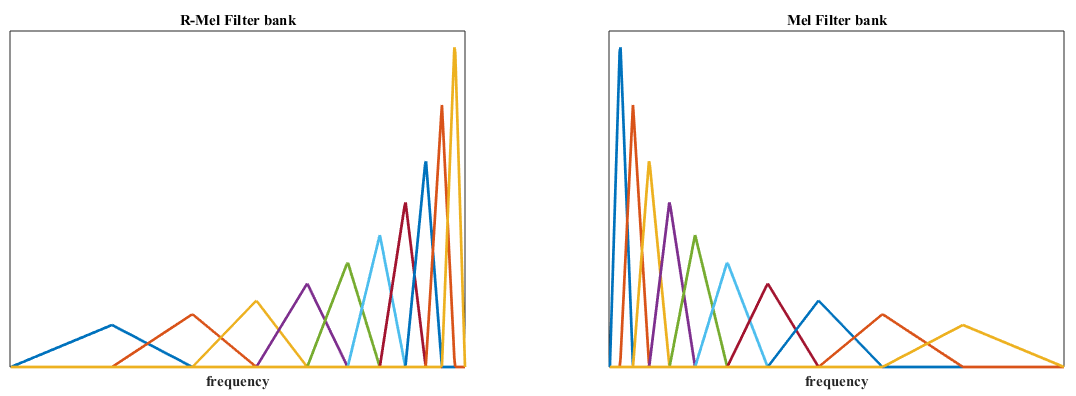
\includegraphics[width=\textwidth,height=0.5\textheight,keepaspectratio]{images/audio-nlp-eval/mel-filter-bank.png}
        \caption*{Mel filter bank. Source: Wikipedia}
    \end{figure}

\end{frame}

\subsection{Log-Mel Features}
\begin{frame}[allowframebreaks]{Log-Mel Features}

\begin{itemize}
    \item Log-Mel features are created by taking the logarithm of mel-band energies:
    \[
        \log(E_m)
    \]
    where $E_m$ is the energy in the $m$-th mel band.

    \item Processing pipeline:
    \begin{itemize}
        \item Compute STFT $\;\rightarrow\;$ apply mel filterbank $\;\rightarrow\;$ mel-band energies.
        \item Apply logarithmic compression, either:
        \[
            \log(E_m) \quad \text{or} \quad \log(1 + \alpha E_m)
        \]
        to avoid issues with very small values.
    \end{itemize}
\framebreak
    \item Why this step matters:
    \begin{itemize}
        \item Human perception of loudness is approximately logarithmic.
        \item Log scaling stabilizes feature magnitudes, preventing loud frames from dominating.
        \item Improves optimization for downstream machine learning models.
    \end{itemize}

    \item Applications:
    \begin{itemize}
        \item Ubiquitous in modern \textbf{TTS systems} (e.g., WaveNet-style neural vocoders).
        \item Widely used in speech recognition pipelines.
        \item References: \texttt{arXiv}, Tacotron 2 project.
    \end{itemize}
\end{itemize}

\end{frame}
